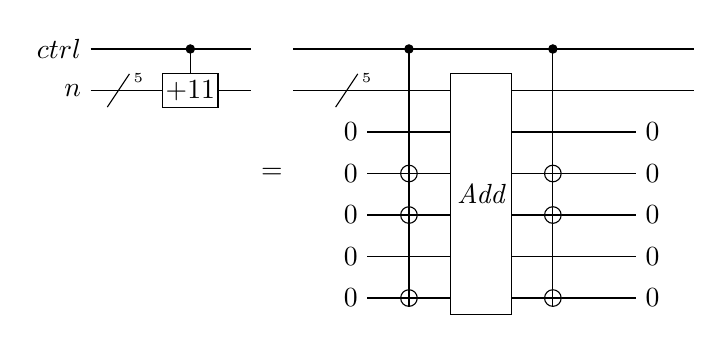
\begin{tikzpicture}[scale=1.000000,x=1pt,y=1pt]
\filldraw[color=white] (0.000000, -7.500000) rectangle (218.000000, 97.500000);
% Drawing wires
% Line 1: ctrl W ctrl
\draw[color=black] (0.000000,90.000000) -- (218.000000,90.000000);
\draw[color=black] (0.000000,90.000000) node[left] {$ctrl$};
% Line 2: n W n
\draw[color=black] (0.000000,75.000000) -- (218.000000,75.000000);
\draw[color=black] (0.000000,75.000000) node[left] {$n$};
% Line 3: m4 W 0 0
\draw[color=black] (92.500000,60.000000) -- (204.500000,60.000000);
% Line 4: m3 W 0 0
\draw[color=black] (92.500000,45.000000) -- (204.500000,45.000000);
% Line 5: m2 W 0 0
\draw[color=black] (92.500000,30.000000) -- (204.500000,30.000000);
% Line 6: m1 W 0 0
\draw[color=black] (92.500000,15.000000) -- (204.500000,15.000000);
% Line 7: m0 W 0 0
\draw[color=black] (92.500000,0.000000) -- (204.500000,0.000000);
% Done with wires; drawing gates
% Line 9: n / ^5
\draw (6.000000, 69.000000) -- (14.000000, 81.000000);
\draw (12.000000, 78.000000) node[right] {$\scriptstyle{^5}$};
% Line 11: n G width=20 $+11$ ctrl
\draw (36.000000,90.000000) -- (36.000000,75.000000);
\begin{scope}
\draw[fill=white] (36.000000, 75.000000) +(-45.000000:14.142136pt and 8.485281pt) -- +(45.000000:14.142136pt and 8.485281pt) -- +(135.000000:14.142136pt and 8.485281pt) -- +(225.000000:14.142136pt and 8.485281pt) -- cycle;
\clip (36.000000, 75.000000) +(-45.000000:14.142136pt and 8.485281pt) -- +(45.000000:14.142136pt and 8.485281pt) -- +(135.000000:14.142136pt and 8.485281pt) -- +(225.000000:14.142136pt and 8.485281pt) -- cycle;
\draw (36.000000, 75.000000) node {$+11$};
\end{scope}
\filldraw (36.000000, 90.000000) circle(1.500000pt);
% Line 13: =
\draw[fill=white,color=white] (58.000000, -6.000000) rectangle (73.000000, 96.000000);
\draw (65.500000, 45.000000) node {$=$};
% Line 15: n / ^5
\draw (88.500000, 69.000000) -- (96.500000, 81.000000);
\draw (94.500000, 78.000000) node[right] {$\scriptstyle{^5}$};
% Line 17: m4 START
\draw[color=black] (100.000000,60.000000) node[fill=white,left,minimum height=15.000000pt,minimum width=15.000000pt,inner sep=0pt] {\phantom{$0$}};
\draw[color=black] (100.000000,60.000000) node[left] {$0$};
% Line 18: m3 START
\draw[color=black] (100.000000,45.000000) node[fill=white,left,minimum height=15.000000pt,minimum width=15.000000pt,inner sep=0pt] {\phantom{$0$}};
\draw[color=black] (100.000000,45.000000) node[left] {$0$};
% Line 19: m2 START
\draw[color=black] (100.000000,30.000000) node[fill=white,left,minimum height=15.000000pt,minimum width=15.000000pt,inner sep=0pt] {\phantom{$0$}};
\draw[color=black] (100.000000,30.000000) node[left] {$0$};
% Line 20: m1 START
\draw[color=black] (100.000000,15.000000) node[fill=white,left,minimum height=15.000000pt,minimum width=15.000000pt,inner sep=0pt] {\phantom{$0$}};
\draw[color=black] (100.000000,15.000000) node[left] {$0$};
% Line 21: m0 START
\draw[color=black] (100.000000,0.000000) node[fill=white,left,minimum height=15.000000pt,minimum width=15.000000pt,inner sep=0pt] {\phantom{$0$}};
\draw[color=black] (100.000000,0.000000) node[left] {$0$};
% Line 22: ctrl +m3 +m2 +m0
\draw (115.000000,90.000000) -- (115.000000,0.000000);
\filldraw (115.000000, 90.000000) circle(1.500000pt);
\begin{scope}
\draw[fill=white] (115.000000, 45.000000) circle(3.000000pt);
\clip (115.000000, 45.000000) circle(3.000000pt);
\draw (112.000000, 45.000000) -- (118.000000, 45.000000);
\draw (115.000000, 42.000000) -- (115.000000, 48.000000);
\end{scope}
\begin{scope}
\draw[fill=white] (115.000000, 30.000000) circle(3.000000pt);
\clip (115.000000, 30.000000) circle(3.000000pt);
\draw (112.000000, 30.000000) -- (118.000000, 30.000000);
\draw (115.000000, 27.000000) -- (115.000000, 33.000000);
\end{scope}
\begin{scope}
\draw[fill=white] (115.000000, 0.000000) circle(3.000000pt);
\clip (115.000000, 0.000000) circle(3.000000pt);
\draw (112.000000, 0.000000) -- (118.000000, 0.000000);
\draw (115.000000, -3.000000) -- (115.000000, 3.000000);
\end{scope}
% Line 23: n m4 m3 m2 m1 m0 G width=22 $\textit{Add}$
\draw (141.000000,75.000000) -- (141.000000,0.000000);
\begin{scope}
\draw[fill=white] (141.000000, 37.500000) +(-45.000000:15.556349pt and 61.518290pt) -- +(45.000000:15.556349pt and 61.518290pt) -- +(135.000000:15.556349pt and 61.518290pt) -- +(225.000000:15.556349pt and 61.518290pt) -- cycle;
\clip (141.000000, 37.500000) +(-45.000000:15.556349pt and 61.518290pt) -- +(45.000000:15.556349pt and 61.518290pt) -- +(135.000000:15.556349pt and 61.518290pt) -- +(225.000000:15.556349pt and 61.518290pt) -- cycle;
\draw (141.000000, 37.500000) node {$\textit{Add}$};
\end{scope}
% Line 24: ctrl +m3 +m2 +m0
\draw (167.000000,90.000000) -- (167.000000,0.000000);
\filldraw (167.000000, 90.000000) circle(1.500000pt);
\begin{scope}
\draw[fill=white] (167.000000, 45.000000) circle(3.000000pt);
\clip (167.000000, 45.000000) circle(3.000000pt);
\draw (164.000000, 45.000000) -- (170.000000, 45.000000);
\draw (167.000000, 42.000000) -- (167.000000, 48.000000);
\end{scope}
\begin{scope}
\draw[fill=white] (167.000000, 30.000000) circle(3.000000pt);
\clip (167.000000, 30.000000) circle(3.000000pt);
\draw (164.000000, 30.000000) -- (170.000000, 30.000000);
\draw (167.000000, 27.000000) -- (167.000000, 33.000000);
\end{scope}
\begin{scope}
\draw[fill=white] (167.000000, 0.000000) circle(3.000000pt);
\clip (167.000000, 0.000000) circle(3.000000pt);
\draw (164.000000, 0.000000) -- (170.000000, 0.000000);
\draw (167.000000, -3.000000) -- (167.000000, 3.000000);
\end{scope}
% Line 25: m4 LABEL
% Line 26: m4 END
\draw[color=black] (197.000000,60.000000) node[fill=white,right,minimum height=15.000000pt,minimum width=15.000000pt,inner sep=0pt] {\phantom{$0$}};
\draw[color=black] (197.000000,60.000000) node[right] {$0$};
% Line 27: m3 END
\draw[color=black] (197.000000,45.000000) node[fill=white,right,minimum height=15.000000pt,minimum width=15.000000pt,inner sep=0pt] {\phantom{$0$}};
\draw[color=black] (197.000000,45.000000) node[right] {$0$};
% Line 28: m2 END
\draw[color=black] (197.000000,30.000000) node[fill=white,right,minimum height=15.000000pt,minimum width=15.000000pt,inner sep=0pt] {\phantom{$0$}};
\draw[color=black] (197.000000,30.000000) node[right] {$0$};
% Line 29: m1 END
\draw[color=black] (197.000000,15.000000) node[fill=white,right,minimum height=15.000000pt,minimum width=15.000000pt,inner sep=0pt] {\phantom{$0$}};
\draw[color=black] (197.000000,15.000000) node[right] {$0$};
% Line 30: m0 END
\draw[color=black] (197.000000,0.000000) node[fill=white,right,minimum height=15.000000pt,minimum width=15.000000pt,inner sep=0pt] {\phantom{$0$}};
\draw[color=black] (197.000000,0.000000) node[right] {$0$};
% Done with gates; drawing ending labels
% Done with ending labels; drawing cut lines and comments
% Done with comments
\end{tikzpicture}
